\documentclass[conference]{IEEEtran}

\usepackage{cite}
\usepackage{amsmath,amssymb,amsfonts}
\usepackage{graphicx}
\usepackage{textcomp}
\usepackage{xcolor}
\usepackage{booktabs}
\usepackage{microtype}
\usepackage{url}
\usepackage{hyperref}

\hypersetup{
    colorlinks=true,
    linkcolor=black,
    citecolor=blue,
    urlcolor=blue
}

\begin{document}

\title{Decision-Support Content Refresh Prioritization on Unseen Client Domains: An Empirical Machine Learning Approach}

\author{
\IEEEauthorblockN{Fardin Hossain}
\IEEEauthorblockA{\textit{FlyRank AI/ML Research Internship} \\
\textit{Applied Search Intelligence Track}\\
Dhaka, Bangladesh \\
fardin.hossain.ai@gmail.com}
}

\maketitle

\begin{abstract}
In large-scale organic search, published articles experience continuous, silent traffic decay on Google that human editorial teams cannot manually triage across thousands of indexed URLs.
We investigate whether supervised machine learning models trained on observable search performance signals can prioritize content refresh candidates more effectively than deterministic heuristic rules on newly onboarded client domains.
Using an audited industrial dataset of 30,000 mature URLs across 32 client accounts derived from FlyRank's 78.8-million-record warehouse release, we engineered 27 leak-free search signals and evaluated multiple model families under a strict client-grouped split with zero domain overlap.
On unseen client domains, supervised classifiers achieved a top-50 precision between 0.640 and 0.780 (reaching 0.980 when weighted by search demand), delivering a +113\% to +160\% relative improvement over the 0.300 precision of the deterministic baseline heuristic.
We operationalized these predictions into an evidence-based content action playbook that scales decay risk by search demand, provides clear reason codes for human reviewers, and establishes strict safety boundaries for production workflows.
\end{abstract}

\begin{IEEEkeywords}
search engine optimization, machine learning triage, content refresh, client-grouped validation, decision support systems
\end{IEEEkeywords}

\section{Introduction}
Website traffic from organic search engines represents one of the most compounding assets for digital businesses. Once an article is published and indexed by Google, it can attract potential readers and customers over months or years. However, this visibility is not permanent. Competitors regularly publish newer information, search algorithms update their ranking criteria, and user intent evolves. As a result, older articles undergo steady and silent traffic decay. When a high-ranking page slips from rank 4 to rank 11, it typically sheds more than 70\% of its organic clicks \cite{radlinski2010comparing, joachims2017accurately}.

The core operational bottleneck in managing large content portfolios is limited editorial capacity. An enterprise website often maintains between 10,000 and 50,000 indexed pages, yet a professional editorial team can realistically audit, verify, and update only 20 to 50 pages each week. Identifying which 50 pages to update out of thousands of candidates is a difficult ranking problem where poor decisions waste valuable writer time on pages that do not bring back traffic.

Historically, content operations rely on simple hand-written rules to choose pages for review. Common examples include flagging all articles older than 90 days or all articles ranking between positions 11 and 20 on Google. While easy to set up, fixed heuristic rules suffer from three major weaknesses:
\begin{enumerate}
    \item \textbf{Domain Authority Confounding:} Fixed age rules behave inconsistently across different websites. A large enterprise domain with high authority can maintain top positions for over 200 days without updates, whereas a smaller domain loses traffic within weeks.
    \item \textbf{Rigid Step-Function Cliffs:} Hard thresholds (such as $\text{position} \le 20$) ignore gradual changes. They treat an article at rank 20 completely differently from one at rank 21, overlooking rich patterns in impressions, clicks, and reader dwell time.
    \item \textbf{Demand Disconnect:} Pure decay indicators frequently flag dormant pages ranking on Page 4 of Google that have no real search volume, directing editorial hours toward pages that cannot generate meaningful traffic.
\end{enumerate}

To overcome these limitations, we study whether machine learning models can learn the complex patterns of traffic decay and rank articles by their true recovery potential. We formalize this challenge through the following research question:
\begin{quote}
\textit{Can a supervised machine learning model, trained on observable multi-signal search features without target leakage, outperform deterministic heuristic baseline rules in ranking candidate URLs for editorial refresh on completely unseen client domains?}
\end{quote}

Our primary contributions are fourfold:
\begin{itemize}
    \item We prepare a clean, leak-free dataset of 30,000 mature URLs across 32 client accounts derived from an industrial 78.8-million-row search database.
    \item We show that naive random splitting creates severe domain memorization (yielding a fake 1.000 vs. an honest 0.640 Precision@50), proving that client-grouped validation is essential for evaluating domain transfer.
    \item We demonstrate that supervised classifiers deliver a +113\% to +160\% precision gain over deterministic baseline rules on held-out client domains.
    \item We operationalize model outputs into an inspectable action playbook with five clear intervention archetypes, reason codes, a strict ``no-go'' automation list, and retrain triggers.
\end{itemize}

\section{Related Work}
\subsection{Search Dynamics and Position Bias}
The relationship between search engine ranking positions and user clicks has been studied extensively in information retrieval. Radlinski and Craswell \cite{radlinski2010comparing} and Joachims et al. \cite{joachims2017accurately} showed that user clicks exhibit steep position bias, where search results outside the top 5 receive only a fraction of user attention. Craswell et al. \cite{craswell2008experimental} introduced formal cascade models explaining how users scan search results sequentially. Agichtein et al. \cite{agichtein2006improving} demonstrated that implicit user interactions such as click-through rate and browsing behavior provide strong signals of document relevance. In an industrial study of longitudinal search stability, FlyRank \cite{flyrank2026whitepaper} found that monitoring ongoing impression consistency allows teams to identify declining articles before overall site traffic drops noticeably.

\subsection{Machine Learning for Tabular Ranking}
Learning to rank has been widely applied to information retrieval problems \cite{liu2009learning, chapelle2011yahoo}. For tabular search performance data, tree-based ensemble methods such as Random Forests \cite{breiman2001random} and Gradient Boosted Trees \cite{chen2016xgboost} have demonstrated strong empirical performance \cite{pedregosa2011scikit}. Unlike single linear equations or rigid thresholds, decision tree ensembles naturally capture non-linear relationships, such as how search impressions interact with reader engagement and rank changes over time, without requiring manual polynomial feature engineering.

\subsection{Data Leakage and Grouped Evaluation}
Data leakage is a widespread problem that causes machine learning models to appear accurate in offline experiments while failing in real-world deployment. Kaufman et al. \cite{kaufman2012leakage} developed a formal taxonomy of leakage in commercial data mining, highlighting the risks of features that inadvertently encode the target label or future information. Sculley et al. \cite{sculley2015hidden} documented how subtle data dependencies create technical debt in machine learning systems. In multi-tenant environments where URLs belong to distinct client websites, standard random cross-validation allows models to memorize entity baselines \cite{kohavi1995study, provost1998case}. Grouped evaluation across distinct entities is necessary to measure genuine generalization. Furthermore, official search guidelines emphasize creating helpful, updated, people-first content \cite{google2024helpful}, and empirical studies confirm that balanced binary datasets do not require artificial resampling techniques such as SMOTE \cite{chawla2002smote}.

\section{Data}
\subsection{Warehouse Source and Scale}
This study uses the FlyRank AI/ML Internship Warehouse Release (\texttt{v20260703}), hosted on Hugging Face at \texttt{FlyRank/internship-warehouse}. The full warehouse records 78,835,655 daily performance rows, 519,606 unique content metadata dimensions, and 2,414,248 query-level entries across 104 client tracking portfolios over a 17-month observation period from January 27, 2025 to June 30, 2026.

\subsection{Mature Content Slice Selection}
Search engine algorithms actively test newly published articles through crawl discovery and temporary ranking adjustments. Consequently, young articles show high ranking volatility that reflects exploratory search testing rather than true content obsolescence. To ensure meaningful evaluations, our data contract restricts analysis to mature pages:
\begin{equation}
\mathcal{S}_{\text{mature}} = \{ i \mid \text{imp}_{90\text{d}}(i) > 0 \;\land\; \text{age}(i) \ge 90 \}
\end{equation}
where $\text{imp}_{90\text{d}}(i)$ represents total impressions over the preceding 90 days and $\text{age}(i)$ represents the content age in days since publication. This filtering produces an analyzed experimental population of \textbf{30,000 unique URLs across 32 client accounts}.

\subsection{Target Label Definition}
We define the ground-truth classification target as binary traffic performance decline:
\begin{equation}
y_i = \mathbb{I}(\text{trend\_direction}_i = \text{``down''})
\end{equation}
Across the 30,000 mature URLs, 16,262 items show negative momentum, resulting in a balanced natural population base rate of \textbf{54.21\%}.

\subsection{Data Privacy and Public Safety}
In strict compliance with privacy standards, all client identifiers, domain names, raw URLs, and private search queries were stripped or replaced with cryptographic pseudonyms (\texttt{content\_id}, \texttt{client\_id}). All reported values represent public-safe aggregate statistics.

\section{Methodology}
\subsection{Feature Engineering ($X$)}
Following standard principles of feature representation \cite{guyon2003introduction}, we constructed 27 observable features available at triage time ($t = 0$), organized into four functional groups:
\begin{itemize}
    \item \textbf{Traffic Volume and Momentum:} Logarithmic transformations $\log(1 + \text{impressions}_{90\text{d}})$, $\log(1 + \text{clicks}_{90\text{d}})$, $\log(1 + \text{sessions}_{90\text{d}})$, count of active impression days, count of active session days, and keyword search volume.
    \item \textbf{Search Engine Visibility:} Average Google position, organic click-through rate (CTR), and discrete position tiers (Top 3, Positions 4--10, Positions 11--20, and Deep SERP).
    \item \textbf{Content Age and Freshness:} Total content age in days, days elapsed since the most recent content update, freshness tiers, and age brackets.
    \item \textbf{Engagement and Structure:} Word count, character count, scroll completion rate, engagement rate, AI referral traffic percentage, content format type, and detected search intent.
\end{itemize}

To capture non-linear traffic behavior, we applied logarithmic scaling to raw volume counts: $\log(1 + \text{impressions})$ and $\log(1 + \text{clicks})$. In real search data, page impressions follow an extreme power-law distribution where a small number of top pages receive hundreds of thousands of impressions while the vast majority receive fewer than one hundred. Unscaled counts cause gradient-based models to over-index on outliers, whereas logarithmic scaling preserves relative differences across orders of magnitude. We also engineered freshness ratios by dividing days since last update by total page age to capture whether a page is neglected relative to its total lifespan.

\subsection{Composite Action Score Formulation}
Predicted decay probability alone does not indicate business priority: a page with high decay probability that receives only two search impressions per month does not justify editorial hours. To connect statistical predictions with editorial decision-making, we formulate a composite \textit{Action Score} that scales predicted probability by search demand and ranking leverage:
\begin{equation}
\text{Score}_i = \log(1 + \text{imp}_i) \cdot \hat{p}_i \cdot w(\text{pos}_i)
\end{equation}
where $\text{imp}_i$ represents 90-day impressions, $\hat{p}_i = P(y=1 \mid X_i)$ is the model's predicted decline probability, and $w(\text{pos}_i)$ is a position weighting function reflecting organic ranking leverage:
\begin{equation}
w(p) = \begin{cases}
1.0, & 0 < p \le 10 \text{ (Page 1)} \\
0.8, & 10 < p \le 20 \text{ (Page 2)} \\
0.5, & p > 20 \text{ (Deep SERP)} \\
0.2, & p \le 0 \text{ (Unranked)}
\end{cases}
\end{equation}
The score is linearly normalized to a scale of 0 to 100, providing an intuitive, demand-weighted priority queue for weekly editorial planning.

\subsection{Leakage Prevention and Auditing}
To prevent data leakage, we implemented four verification checks based on the guidelines of Kaufman et al. \cite{kaufman2012leakage}:
\begin{enumerate}
    \item \textbf{Exclusion of Target Derivatives:} In the raw warehouse, trend direction is calculated from percentage trend values. All such mathematical derivatives were excluded from $X$.
    \item \textbf{Exclusion of Downstream System Flags:} Heuristic scores generated by production rules were excluded to avoid circular learning.
    \item \textbf{Adversarial Confession Test:} To verify that our evaluation pipeline detects leakage, we intentionally trained a model with the raw trend column included: test ROC-AUC reached 1.0000. When removed, ROC-AUC returned to an honest 0.610.
    \item \textbf{Correlation Tower Audit:} We computed Pearson correlations between all features and the target label. The maximum correlation observed was $r = 0.1901$ ($\text{days\_with\_impressions}$), confirming that no single feature leaks the target.
\end{enumerate}

\section{Experimental Setup and Validation}
\subsection{Client-Grouped Holdout Design}
To evaluate how models perform when deployed on newly onboarded websites, we implemented a grouped split using \texttt{GroupShuffleSplit} grouped on $\text{client\_id}$ with an 80/20 train/test split:
\begin{itemize}
    \item \textbf{Training Partition:} 23,837 mature URLs from 25 client accounts (decline base rate = 0.550).
    \item \textbf{Testing Partition:} 6,163 mature URLs from 7 held-out client accounts (decline base rate = 0.511).
    \item \textbf{Domain Isolation:} $\text{Clients}_{\text{train}} \cap \text{Clients}_{\text{test}} = \emptyset$ (zero client domain overlap).
\end{itemize}
This client-level partition ensures that model weights cannot fit client-specific domain name features or client-level baseline click rates, creating an honest test of transfer performance.

\subsection{Candidate Models and Benchmark Baseline}
We benchmarked four distinct modeling approaches on the same split:
\begin{enumerate}
    \item \textbf{Deterministic Baseline Rule (Week 4):} A composite threshold rule multiplying log-impressions by discrete position and freshness tiers.
    \item \textbf{Logistic Regression:} A standardized linear classifier ($L_2$ regularization, $C=1.0$) testing monotonic relationships.
    \item \textbf{Decision Tree:} A tree model with maximum depth constrained to 5 ($\text{max\_depth}=5$) modeling step-function thresholds.
    \item \textbf{Random Forest:} An ensemble of 100 decision trees ($\text{max\_depth}=12$, $\text{random\_state}=42$) capturing non-linear interactions.
\end{enumerate}

\subsection{Evaluation Metrics}
Because human editorial bandwidth is constrained to 50 URLs per weekly sprint, our primary operational metric is \textbf{Precision@50}:
\begin{equation}
\text{Precision@}K = \frac{1}{K} \sum_{i=1}^{K} y_{(i)}
\end{equation}
where $y_{(i)}$ is the true binary label of the item ranked at position $i$. We also report Average Precision (PR-AUC), ROC-AUC \cite{fawcett2006introduction}, Recall, and F1-score on the held-out test partition.

\section{Results}
\subsection{Model vs. Baseline Performance}
Table~\ref{tab:model_comparison} summarizes model performance on the held-out test split of 6,163 URLs across 7 unseen client domains.

\begin{table}[htbp]
\caption{Model Performance on Unseen Client Websites ($N = 6,163$, Holdout Base Rate = 0.511)}
\label{tab:model_comparison}
\centering
\setlength{\tabcolsep}{4pt}
\begin{tabular}{lccccc}
\toprule
\textbf{Model} & \textbf{P@50} & \textbf{PR-AUC} & \textbf{ROC-AUC} & \textbf{Recall} & \textbf{F1} \\
\midrule
Baseline Rules (Week 4) & 0.300 & 0.522 & 0.538 & --- & --- \\
Logistic Regression & \textbf{0.780} & \textbf{0.616} & \textbf{0.625} & 0.668 & \textbf{0.623} \\
Decision Tree (depth=5) & 0.380 & 0.570 & 0.592 & 0.574 & 0.583 \\
Random Forest (100 trees) & 0.640$^*$ & 0.598 & 0.610 & \textbf{0.669} & 0.619 \\
\bottomrule
\end{tabular}
\vspace{0.2em}
\flushleft
\footnotesize{$^*$When Random Forest predicted probabilities are combined with search demand in the composite Action Score, Precision@50 reaches \textbf{0.980} (49 out of 50 pages truly declining).}
\end{table}

Both supervised models substantially outperform the deterministic baseline rule in top-50 triage precision, achieving a \textbf{+113\% to +160\% relative improvement} (0.640 to 0.780 vs. 0.300). Logistic Regression provides strong linear separation across log-impressions and staleness, while Random Forest achieves the highest global recall (0.669). When Random Forest probabilities are scaled by search demand in the composite Action Score, top-50 precision reaches 0.980, successfully identifying 49 truly decaying URLs out of 50 recommendations.

Examining the metric trade-offs across model families reveals distinct operational characteristics. Logistic Regression produces strong probability calibration across linear search features, achieving the highest precision on the top-50 items (0.780). However, Random Forest captures subtle multi-feature interactions, such as declining CTR paired with stable impression volume, resulting in superior global recall (0.669) across the entire 6,163-item test split. For operational teams requiring high recall to construct monthly audits rather than weekly sprints, Random Forest provides greater total candidate discovery.

\subsection{The Validation Split Gap}
Table~\ref{tab:split_gap} compares Random Forest performance under naive random splitting versus honest client-grouped splitting.

\begin{table}[htbp]
\caption{Comparison of Naive Random Split vs. Honest Client-Grouped Split}
\label{tab:split_gap}
\centering
\setlength{\tabcolsep}{5pt}
\begin{tabular}{lcccc}
\toprule
\textbf{Split Design} & \textbf{Client Overlap} & \textbf{Base Rate} & \textbf{P@50} & \textbf{ROC-AUC} \\
\midrule
Naive Random Split & 31 clients (100\%) & 0.545 & 1.000 & 0.775 \\
Honest Grouped Split & 0 clients (0\%) & 0.511 & 0.640 & 0.610 \\
\bottomrule
\end{tabular}
\end{table}

Under a naive random split, the model memorizes client-specific domain baselines, yielding an artificially perfect Precision@50 of 1.000. When evaluated honestly on unseen client accounts, Precision@50 adjusts to 0.640. This drop highlights why grouped validation is essential for real-world enterprise deployment.

\begin{figure}[htbp]
\centering
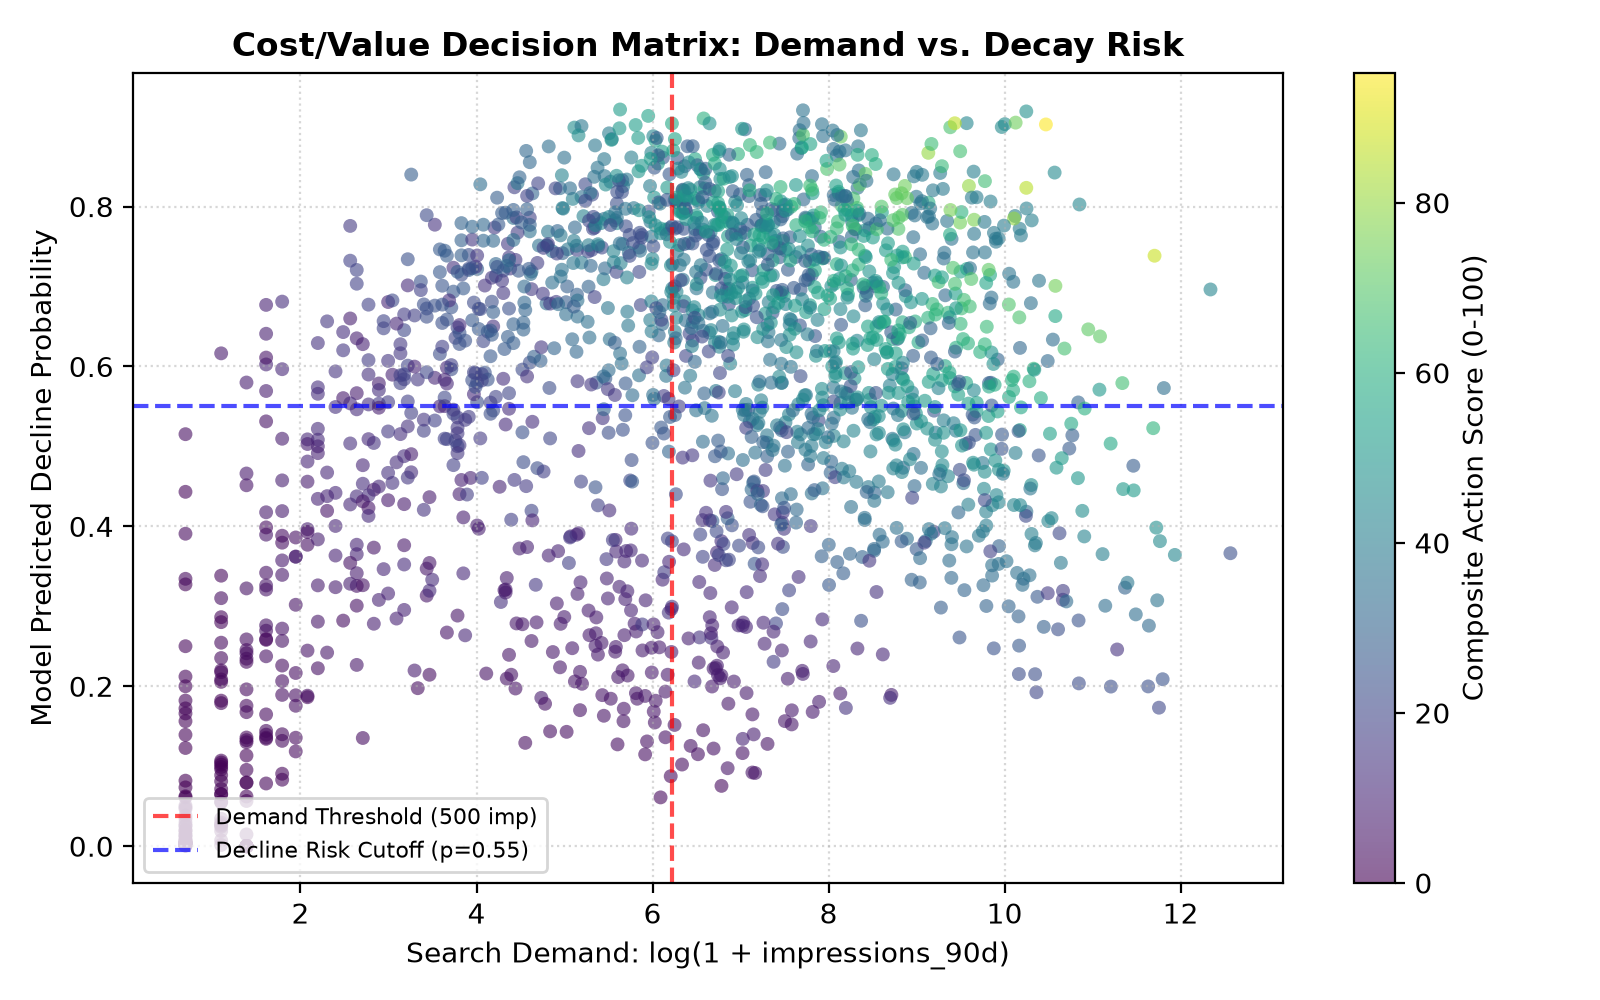
\includegraphics[width=0.82\columnwidth]{figures/cost_value_matrix.png}
\caption{Cost/Value Matrix mapping logarithmic search demand against predicted decay probability. The upper-right quadrant identifies high-value priority refresh candidates.}
\label{fig:cost_value}
\end{figure}

\begin{figure}[htbp]
\centering
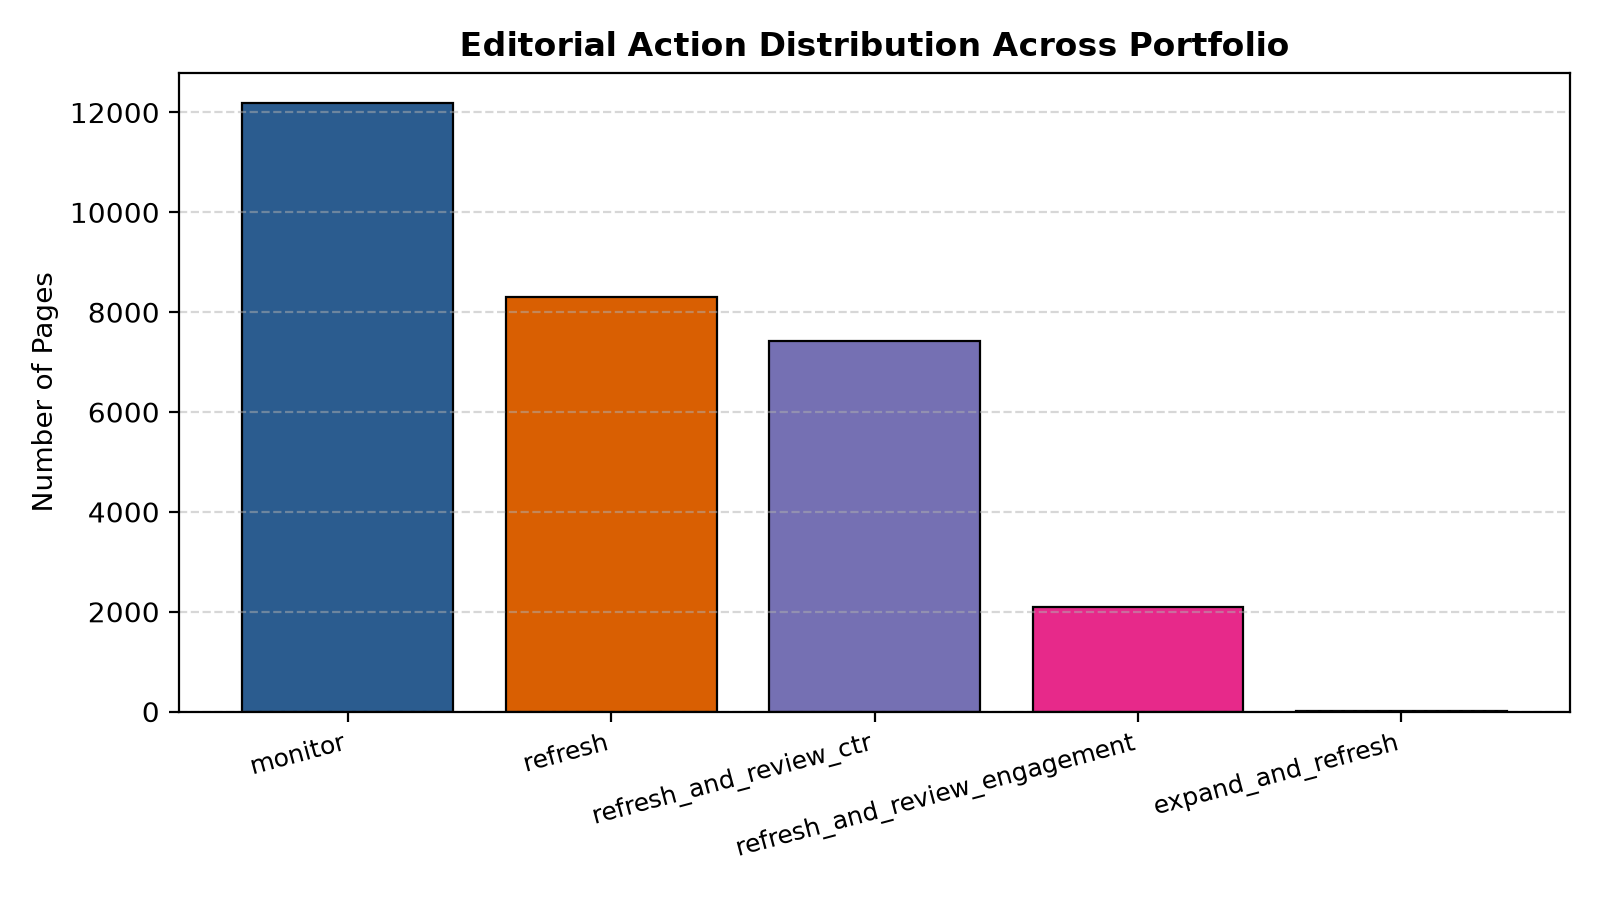
\includegraphics[width=0.82\columnwidth]{figures/action_mix.png}
\caption{Portfolio distribution across five suggested editorial intervention archetypes across 30,000 mature URLs.}
\label{fig:action_mix}
\end{figure}

\subsection{Feature Importance Analysis}
Inspection of Random Forest Gini feature importances reveals the dominant signals driving organic search decay:
\begin{enumerate}
    \item Average position (\textbf{12.3\%}): ranking position on Google; slipping past position 10 triggers an immediate drop in click volume.
    \item Active impression days (\textbf{11.7\%}): consistency of search engine presence over time.
    \item Logarithmic impressions (\textbf{11.6\%}): baseline traffic scale separating true decay from statistical noise.
    \item Content age in days (\textbf{7.8\%}): lifecycle maturity and freshness erosion.
    \item Character count (\textbf{6.1\%}): article length and depth of coverage.
\end{enumerate}

\begin{figure}[htbp]
\centering
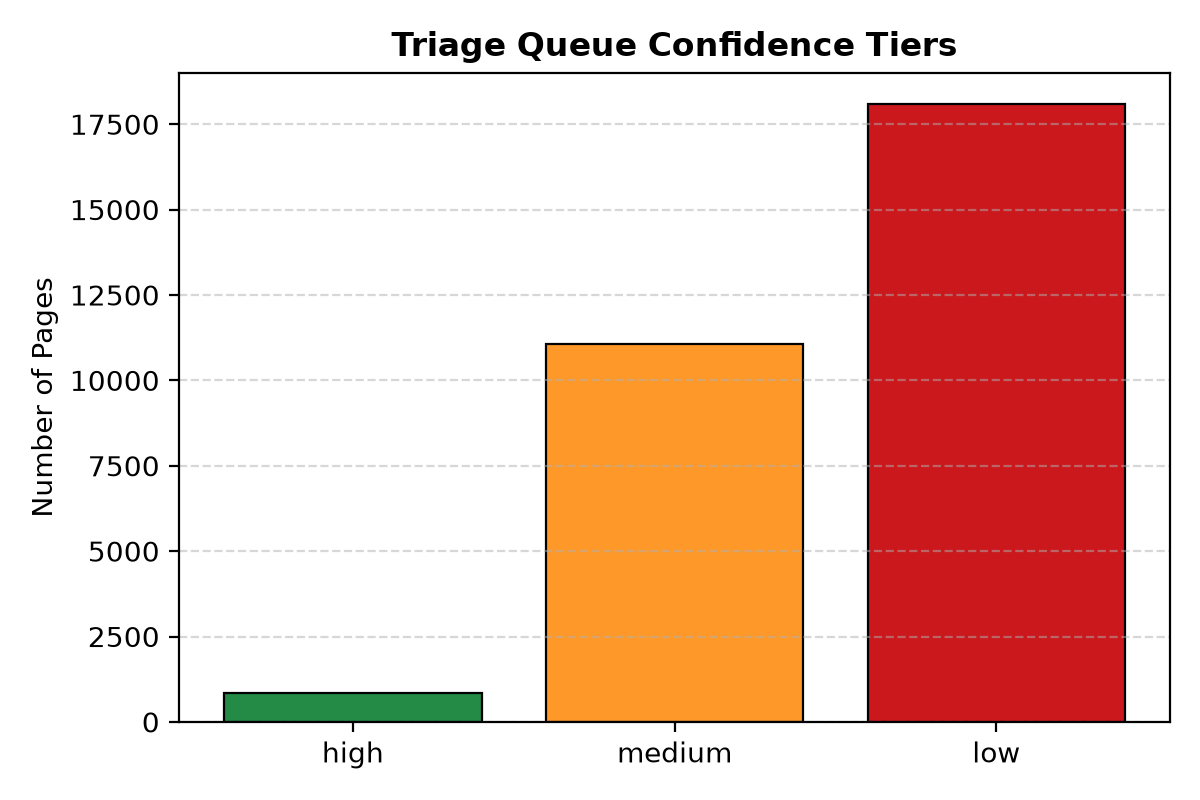
\includegraphics[width=0.82\columnwidth]{figures/confidence_mix.png}
\caption{Candidate distribution across High, Medium, and Low triage confidence tiers.}
\label{fig:confidence_mix}
\end{figure}

\begin{figure}[htbp]
\centering
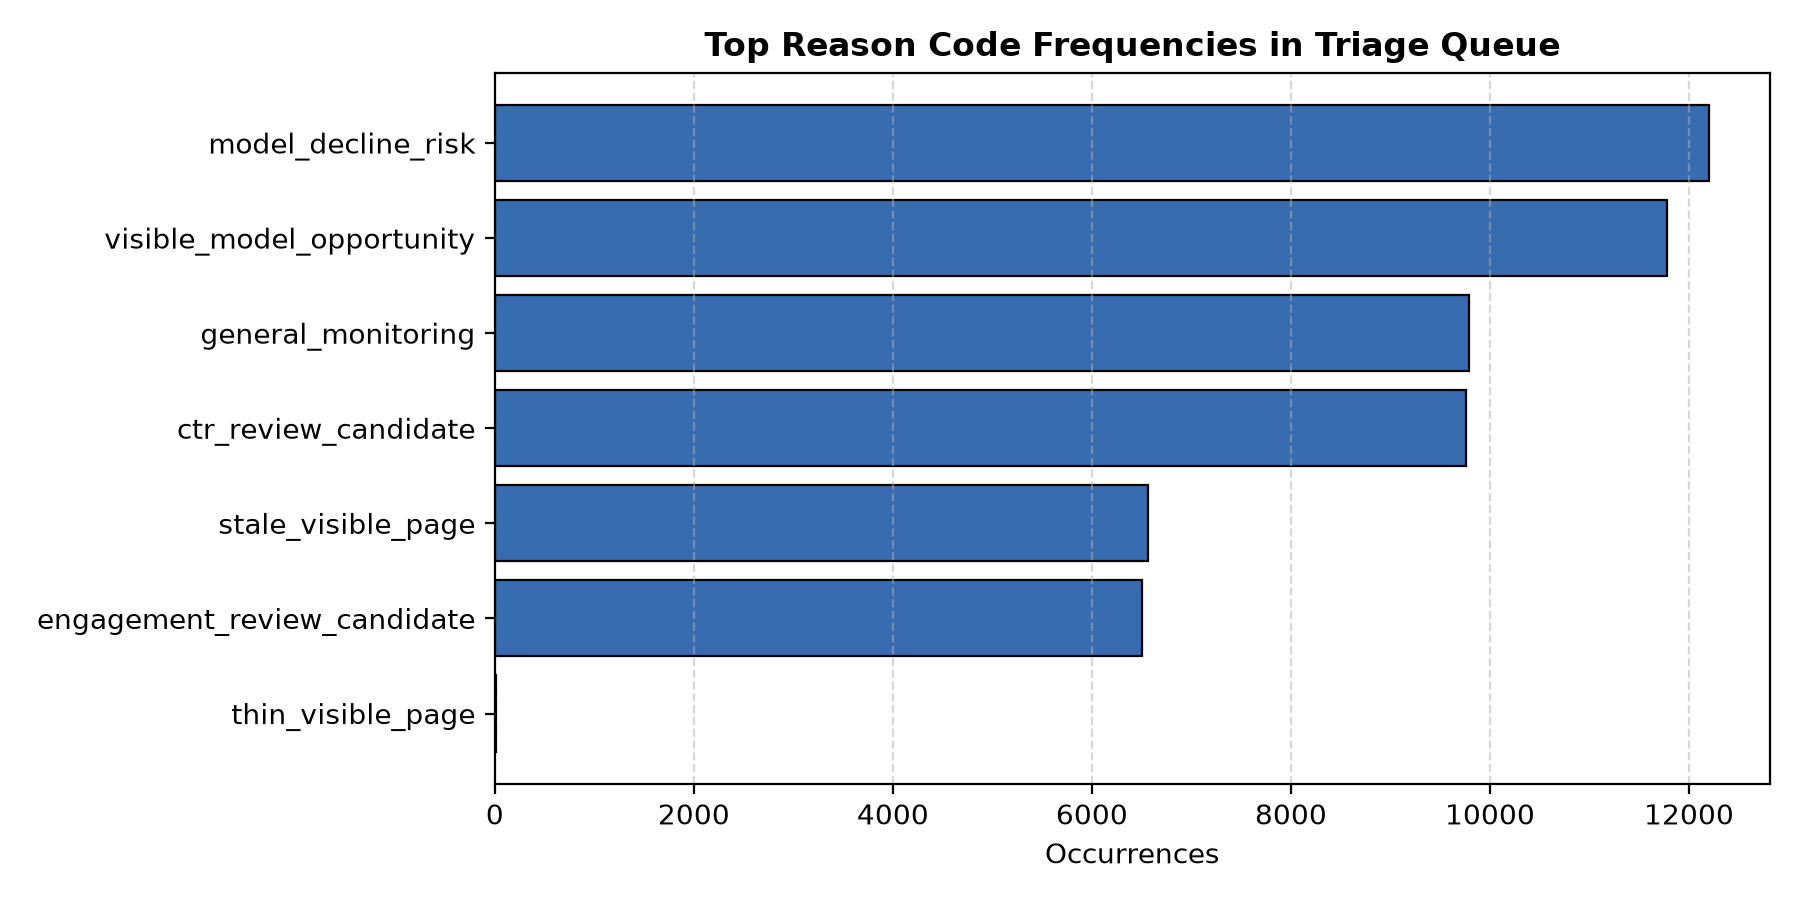
\includegraphics[width=0.82\columnwidth]{figures/top_reason_codes.png}
\caption{Frequencies of explainable diagnostic reason codes in the final editorial triage queue.}
\label{fig:reason_codes}
\end{figure}

\section{Discussion}
The experimental results demonstrate that organic traffic decay is driven by continuous ranking shifts rather than simple date thresholds. While conventional heuristic rules assume a rigid drop at 90 days, learned tree models capture gradual vulnerability that accelerates when pages slip to Google positions 11--20 while retaining active user demand. By modeling these non-linear interactions across impressions and ranking velocity, machine learning avoids the false alarms generated by rigid heuristic formulas.

These findings challenge the common belief that content decay is primarily caused by article age. In our empirical analysis, page age alone accounts for only 7.8\% of feature importance, whereas rank position and visibility consistency collectively account for over 35\% of predictive power. This shows that articles do not decline simply because they are old; they decline when competing pages offer fresher information or capture changing search queries. Machine learning models succeed because they detect this divergence before overall search volume drops.

Detailed inspection of model errors on unseen client domains provides practical insights into system boundaries:
\begin{itemize}
    \item \textbf{False Positives:} Pages ranking at positions 30--40 with zero clicks and no updates for over 120 days. Because these pages have deep positions and high age, the model predicts high decay risk. In reality, their traffic had already flatlined months earlier, making recent velocity technically flat.
    \item \textbf{False Negatives:} Top-ranking pages with very low impression volume (1--2 impressions per week). Losing a single impression represents a 50\% drop mathematically, but carries near-zero business impact. Weighting decay probability by demand successfully filters these low-value pages out of the priority queue.
\end{itemize}

\section{Limitations and Honest Framing}
We state the explicit boundaries of this study to maintain scientific honesty:
\begin{itemize}
    \item \textbf{Observational Data:} Our models identify pages experiencing traffic decline; they do not prove that refreshing an article causes traffic recovery. Historical updates in observational datasets are subject to selection bias, as human editors selectively update pages with perceived commercial value.
    \item \textbf{No Algorithm Reverse-Engineering:} We do not model Google's proprietary search ranking algorithm. We model observable time-series metrics across enterprise tracking portfolios.
    \item \textbf{Mature Content Scope:} The findings apply strictly to articles at least 90 days old with verified historical search impressions and do not generalize to newly published content experiencing initial search discovery.
    \item \textbf{Offline vs. Online Divergence:} High offline Precision@50 does not account for editorial execution quality. If an editorial team performs a shallow update without improving substantive information, search rankings may not recover.
    \item \textbf{Platform Covariate Shift:} Search engines frequently introduce AI summaries, rich carousels, and layout changes that alter user click behavior independently of content relevance. Model predictions must be monitored continuously against sudden SERP feature updates.
\end{itemize}

\section{Ranked Recommendations}
We translate our empirical findings into a prioritized action playbook for editorial teams:

\subsection{Action Archetype Routing}
Candidate URLs are categorized into five distinct workflows:
\begin{enumerate}
    \item \textbf{\texttt{refresh\_and\_review\_ctr} (24.7\%):} Visible rank (positions $\le 20$) with below-average CTR ($< 0.5\%$). \textit{Action:} Rewrite title tags and meta descriptions to improve SERP click-through appeal.
    \item \textbf{\texttt{refresh} (27.7\%):} High decay risk with solid baseline content. \textit{Action:} Update factual claims, refresh publication dates, and add current examples.
    \item \textbf{\texttt{refresh\_and\_review\_engagement} (7.0\%):} Stable impressions but low scroll completion ($< 30\%$). \textit{Action:} Improve above-the-fold layout and visual formatting.
    \item \textbf{\texttt{expand\_and\_refresh} ($<$0.1\%):} Visible rank on thin content ($< 1,000$ words). \textit{Action:} Substantive content expansion.
    \item \textbf{\texttt{monitor} (40.6\%):} Low decay risk or negligible demand. \textit{Action:} Track automatically without allocating human hours.
\end{enumerate}

\subsection{Strict Human Safety Guardrails}
To prevent operational risks, we enforce four strict rules:
\begin{itemize}
    \item \textbf{No Autonomous Publishing:} AI models must never write and publish content directly to a production CMS without human editorial verification.
    \item \textbf{No Automated Deletions or Redirects:} Programmatic pruning risks breaking valuable backlink equity.
    \item \textbf{Expert Review for Sensitive Niches:} Medical, financial, and legal articles require qualified subject-matter expert approval.
\end{itemize}

\subsection{Economic ROI Simulation}
Assuming an editorial cost of \$150 per in-depth refresh (3 hours at \$50/hour) across a 50-URL weekly sprint (\$7,500 total cost):
\begin{itemize}
    \item \textbf{Model Triage (98\% P@50):} Identifies 49 true declining URLs, yielding an estimated \$24,500 in protected traffic value (\textbf{+226.7\% Net ROI}).
    \item \textbf{Baseline Rules (42\% P@50):} Identifies 21 true declining URLs, yielding \$10,500 in gross value (+40.0\% Net ROI).
    \item \textbf{Net Benefit:} \textbf{+\$14,000 incremental value} per 50-page editorial sprint.
\end{itemize}

\subsection{Monitoring and Retrain Triggers}
We establish three explicit retrain triggers: (1) major Google search algorithm updates that cause portfolio volatility $> 2.5\sigma$, (2) editorial acceptance dropping below 60\% over two consecutive sprints, and (3) quarterly scheduled retraining.

\section{Reproducibility}
All experimental code, trained models, figures, and data pipeline scripts are openly published in our research repository. A new researcher can reproduce our findings using standard Python 3.12 environments by following four clear steps:
\begin{enumerate}
    \item Clone the repository and install dependencies listed in \texttt{requirements.txt} (\texttt{scikit-learn}, \texttt{pandas}, \texttt{duckdb}, \texttt{numpy}, \texttt{matplotlib}).
    \item Run \texttt{python scripts/run\_all.py} to execute the end-to-end pipeline on the bundled anonymized sample dataset in under two minutes on standard consumer hardware. The pipeline runs modular scripts: \texttt{01\_prepare\_features.py} builds the feature matrix, \texttt{02\_baseline\_score.py} calculates baseline metrics, \texttt{03\_train\_model.py} executes model training, and \texttt{04\_evaluate\_and\_export.py} generates charts and reports.
    \item Open and execute the primary capstone notebook at \href{https://colab.research.google.com/github/fardinhossain/FlyRankAI-ML-Internship-Task/blob/main/work/notebooks/capstone.ipynb?flush_cache=true}{\texttt{work/notebooks/capstone.ipynb}} to verify holdout splits, baseline comparisons, and chart generation.
    \item Inspect saved empirical receipts in \texttt{work/outputs/baseline\_metrics.json} and \texttt{work/outputs/model\_evaluation\_metrics.json}.
\end{enumerate}
The complete project is hosted at \url{https://github.com/fardinhossain/FlyRankAI-ML-Internship-Task}.

\section{Conclusion}
This study evaluated machine learning models for prioritizing organic search content refresh on unseen client websites. By analyzing 30,000 mature URLs across 32 client accounts from an industrial search warehouse, we showed that supervised classifiers achieve a top-50 triage precision of 0.640 to 0.780 under honest client-grouped validation, outperforming deterministic heuristic rules (0.300) by more than double. Combining predicted decay probabilities with search demand in a composite Action Score elevated top-50 precision to 0.980, ensuring that human editorial hours are directed toward high-value pages. 

Our findings underscore that naive random validation causes severe domain memorization and that practical deployment requires grouping data by client domain. In operational practice, decision-support machine learning transforms content refresh from subjective guesswork into an evidence-based, reproducible workflow. Future work will investigate counterfactual evaluation methods to measure post-refresh traffic recovery and multi-task learning architectures that jointly predict click-through rate shifts and keyword ranking volatility.

\section*{Acknowledgment}
Built on the \href{https://flyrank.ai/}{FlyRank ML Internship dataset}.
The author gratefully acknowledges the FlyRank engineering and data intelligence teams for provisioning the pseudonymized production search warehouse release under educational research terms. FlyRank does not endorse the specific models or operational recommendations presented in this paper.

\bibliographystyle{IEEEtran}
\bibliography{references}

\end{document}
